\documentclass{report}
\usepackage[spanish]{babel}
\usepackage[utf8]{inputenc}
\usepackage{graphicx, longtable, float}

\begin{document}

    \begin{titlepage}
        \centering
        
\includegraphics[width=0.6\textwidth]{./img/portada/logo.jpg}\\
        \vspace{1cm}
        \LARGE Análisis y Diseño de Sistemas de Información\\
        \vspace{0.5cm}
        \Large Ingeniería Informática de Gestión y Sistemas de Información\\
        \vspace{3cm}
        \Huge Biblioteca\\
        \vspace{2.5cm}
        \Large Autores:\\
        \vspace{0.2cm}
        \large Xabier Gabiña Barañano\\
        \large Janire Veganzones García\\
        \large Ainhize Martinez Duran\\
        \large Javier Criado Garcia\\
        \large Kepa Reches Urrutia\\
        \large Jon Valdes Granado\\
        \large Mohammed El Basri Dehbi\\
        \vfill
        \today
    \end{titlepage}

    \tableofcontents
    \chapter{Changelog}
        \section{Versión 1 (2023-10-08)}
            \begin{itemize}
                \item Añadido caso de uso general
                \item Añadidos los casos de uso extendidos
            \end{itemize}   
    \chapter{Introducción}
    En un mundo cada vez más digitalizado, las bibliotecas modernas están buscando formas innovadoras de adaptarse a las necesidades cambiantes de sus usuarios. La biblioteca que nos ocupa se encuentra en este proceso de transformación, reconociendo la importancia de expandir sus servicios en línea y brindar a sus usuarios una experiencia más enriquecedora y conectada. Para llevar a cabo esta ambiciosa misión, han solicitado la colaboración de nuestro equipo de desarrollo.\\
    En su estado actual, la biblioteca cuenta con un servicio web que permite a los usuarios consultar su extenso catálogo de libros. Además, ofrece un apartado de usuarios que pueden acceder a una sección privada. Sin embargo, esta plataforma carece de funcionalidades adicionales que pueden mejorar significativamente la experiencia de los usuarios y promover una mayor interacción entre ellos.\\
    En este proyecto, nuestro objetivo es expandir y mejorar el servicio web de la biblioteca, dotándolo de una serie de funcionalidades clave. Estas nuevas características incluyen la gestión de reservas, la capacidad de dejar reseñas y comentarios en los libros, la creación de una red de amigos entre los usuarios, la introducción de un rol de administrador con capacidades de gestión, la implementación de foros para discusión y la incorporación de sistemas de recomendación, tanto basados en el historial de lecturas como en la afinidad de intereses entre usuarios.\\
    A lo largo de este documento, exploraremos en detalle cada una de estas funcionalidades, presentando soluciones técnicas y estratégicas para su implementación. Este proyecto representa una emocionante oportunidad para ayudar a la biblioteca a evolucionar y brindar un servicio en línea más completo y enriquecedor a su comunidad de usuarios ávidos de conocimiento y lectura.\\
    \chapter{Casos de Uso}
        \section{General}
            \begin{figure}[H]
                \centering
                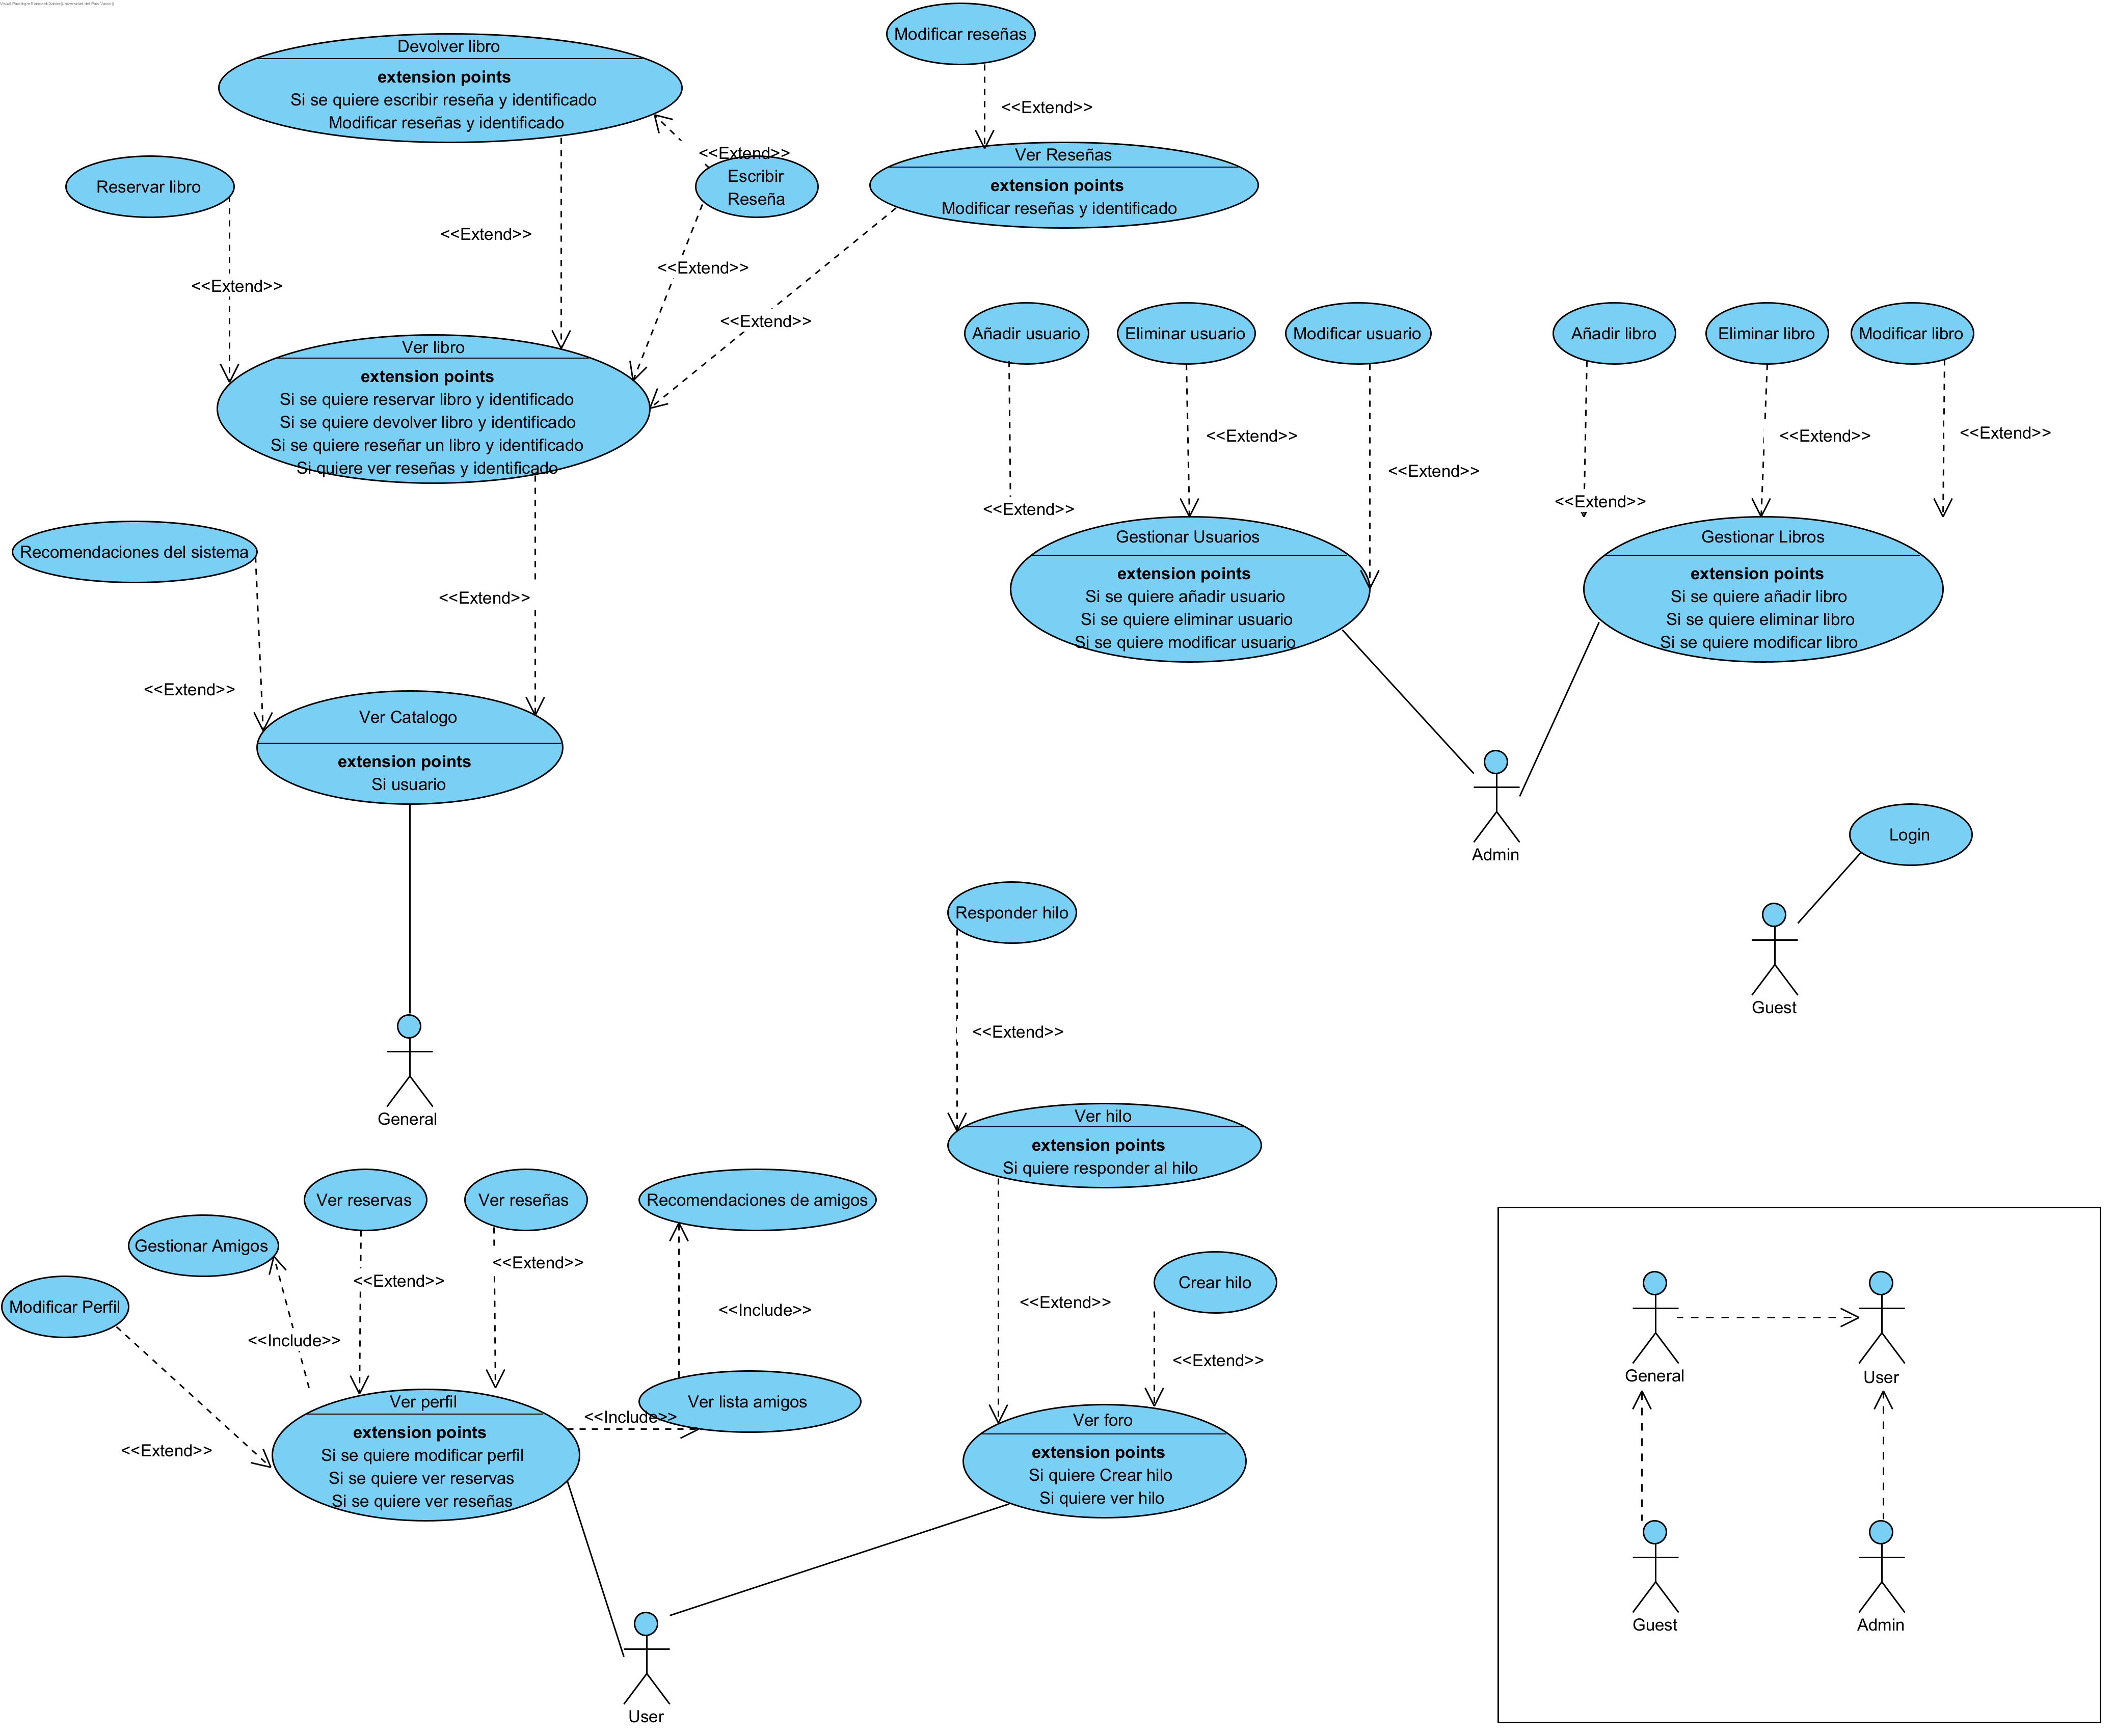
\includegraphics[scale=0.3]{img/casos_uso/General.png}
                \caption{Diagrama de casos de uso general}
            \end{figure}
        \clearpage
        \section{Extendidos}

        \subsection{Gestión de reservas}
            \begin{center}
                \begin{longtable}{|p{\linewidth}|}
                    \hline
                    \textbf{Responsable:} Mohamed El Basri\\
                    \hline
                    \begin{figure}[H]
                        \centering
                        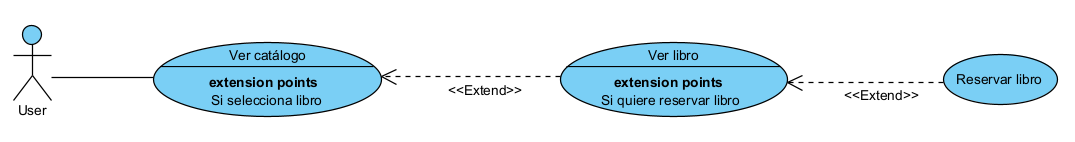
\includegraphics[width=0.8\textwidth]{./img/casos_uso/CasoDeUso_GestionDeReservas.PNG}
                    \end{figure}\\
                    \hline
                    \textbf{Nombre:} Ver libros recomendados\\
                    \hline
                    \textbf{Descripción:} Permite al usuario realizar una reserva de libro.\\
                    \hline
                    \textbf{Actores:} Usuario\\
                    \hline
                    \textbf{Precondiciones:} Estar identificado en el sistema.\\
                    \hline
                    \textbf{Requisitos no funcionales:} Ninguno\\
                    \hline
                    \textbf{Flujo de Eventos:}
                    \begin{enumerate}
                        \item El usuario selecciona el libro deseado en el catálogo y pulsa “Reservar”. Se abre la interfaz de reserva (Ilustración 1).
                        \item Si el usuario pulsa aceptar, si el tiempo de reserva es menor a 2 meses aparece una interfaz indicando que la reserva se ha realizado con éxito (Ilustración 2).
                        \item Si el usuario pulsa aceptar, si el tiempo de reserva es mayor a 2 meses aparece una interfaz indicando error (Ilustración 3).
                        \item Si el usuario pulsa cancelar, se cierra la interfaz.
                    \end{enumerate}\\
                    \hline
                    \textbf{Poscondiciones:} Ninguna\\
                    \hline
                    \textbf{Interfaz Gráfica:}\\
                    \begin{figure}[H]
                        \centering
                        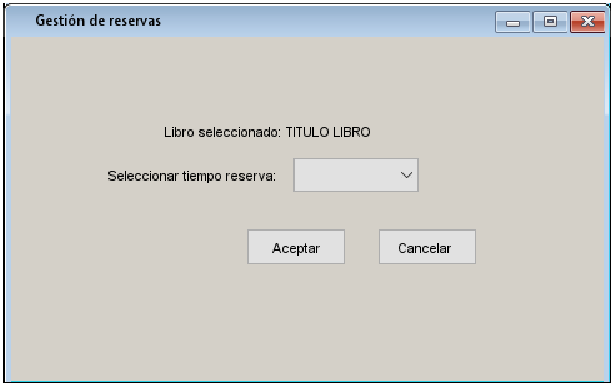
\includegraphics[width=0.8\textwidth]{./img/grafico/GestionDeReservas1.PNG}
                    \end{figure}\\
                    \begin{figure}[H]
                        \centering
                        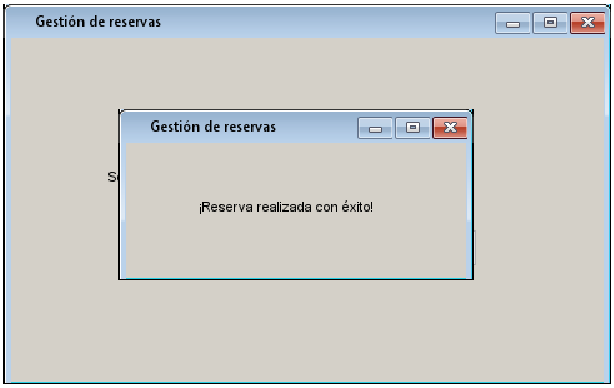
\includegraphics[width=0.8\textwidth]{./img/grafico/GestionDeReservas2.PNG}
                    \end{figure}\\
                    \begin{figure}[H]
                        \centering
                        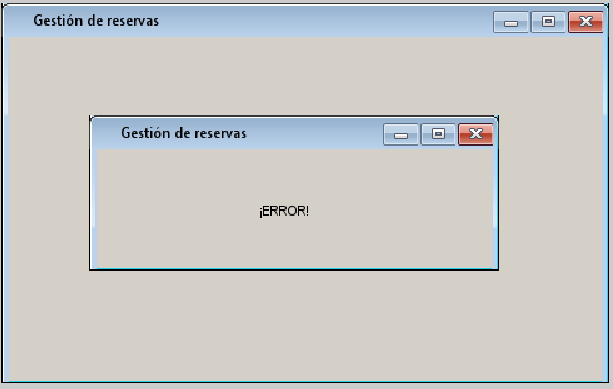
\includegraphics[width=0.8\textwidth]{./img/grafico/GestionDeReservas3.PNG}
                    \end{figure}\\
                    \hline
                \end{longtable}
            \end{center}
        \clearpage

        \subsection{Reseñas}
        \begin{center}
            \begin{longtable}{|p{\linewidth}|}
                \hline
                \textbf{Responsable:} Javier Criado\\
                \hline
                \begin{figure}[H]
                    \centering
                    \includegraphics[width=0.8\textwidth]{./img/casos_uso/Reseñas.jpg}
                \end{figure}\\
                \hline
                \textbf{Nombre:} Reseñas\\
                \hline
                \textbf{Descripción:} Permite al cliente puntuar y comentar en un libro una vez lo haya devuelto, también permite modificar estos datos posteriormente.\\
                \hline
                \textbf{Actores:} Usuario\\
                \hline
                \textbf{Precondiciones:} Estar identificado en el sistema\\
                \hline
                \textbf{Requisitos no funcionales:} Ninguno\\
                \hline
                \textbf{Flujo de Eventos:}
                \begin{enumerate}
                    \item El Usuario entra en el catalogo para ver las peliculas disponibles.
                    \item El usuario selecciona uno de los libros.
                    \item Al seleccionar el boton "Ver reseñas", el usuario podrá ver las reseñas sobre el libro
                    \item Al seleccionar "Devolver libro", se devolvera el libro y se podra añadir una nueva reseña
                    \item Al seleccionar "Escribir reseña", se abrira una pestaña donde se podrá escribir una reseña sobre el libro  
                \end{enumerate}\\
                \hline
                \textbf{Poscondiciones:} Ninguna\\
                \hline
                \textbf{Interfaz Gráfica:}\\
                \begin{figure}[H]
                    \centering
                    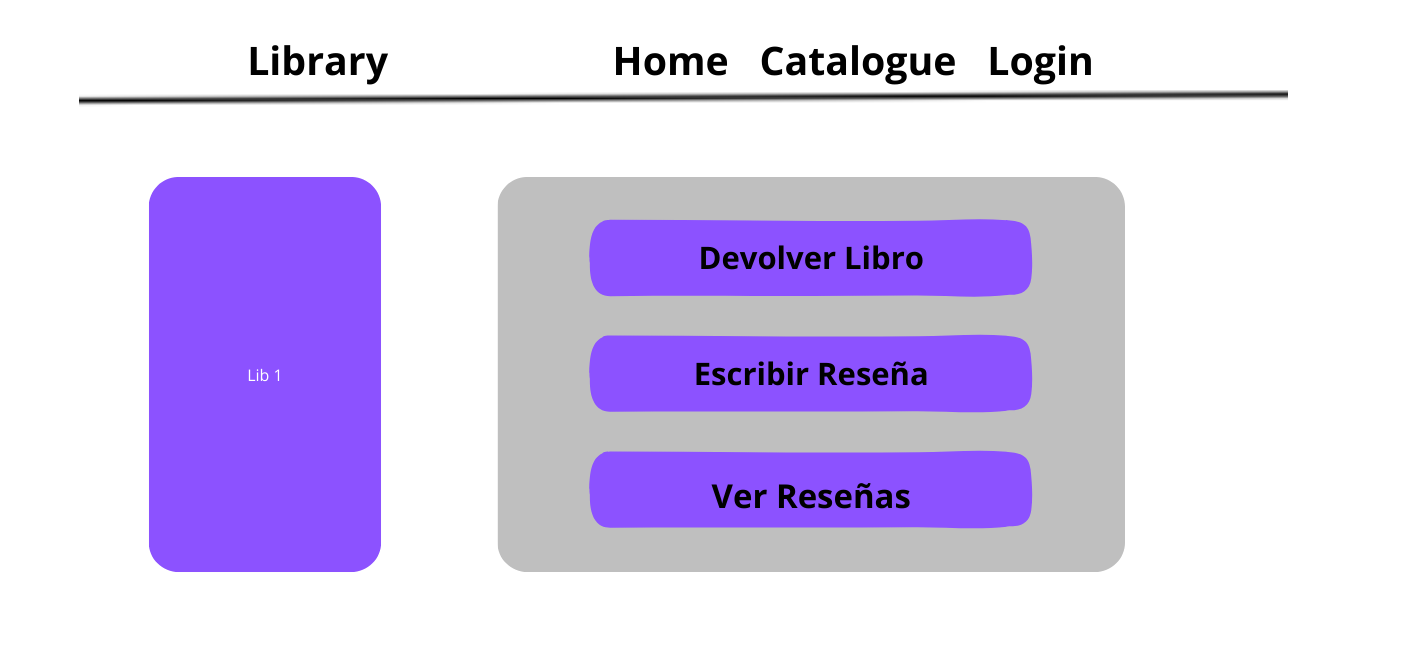
\includegraphics[width=0.8\textwidth]{./img/grafico/Ver_Libro.png}
                \end{figure}\\
                \hline
                \begin{figure}[H]
                    \centering
                    \includegraphics[width=0.8\textwidth]{./img/grafico/Escribir_Reseña.png}
                \end{figure}\\
                \hline
                \begin{figure}[H]
                    \centering
                    \includegraphics[width=0.8\textwidth]{./img/grafico/Ver_Una_Reseña.png}
                \end{figure}\\
                \hline
                \begin{figure}[H]
                    \centering
                    \includegraphics[width=0.8\textwidth]{./img/grafico/Ver_Reseñas.png}
                \end{figure}\\
                \hline
            \end{longtable}
        \end{center}
        \clearpage
        \subsection{Red de amigos}
        \begin{center}
            \begin{longtable}{|p{\linewidth}|}
                \hline
                \textbf{Responsable:} Jon Valdes\\
                \hline
                \begin{figure}[H]
                    \centering
                    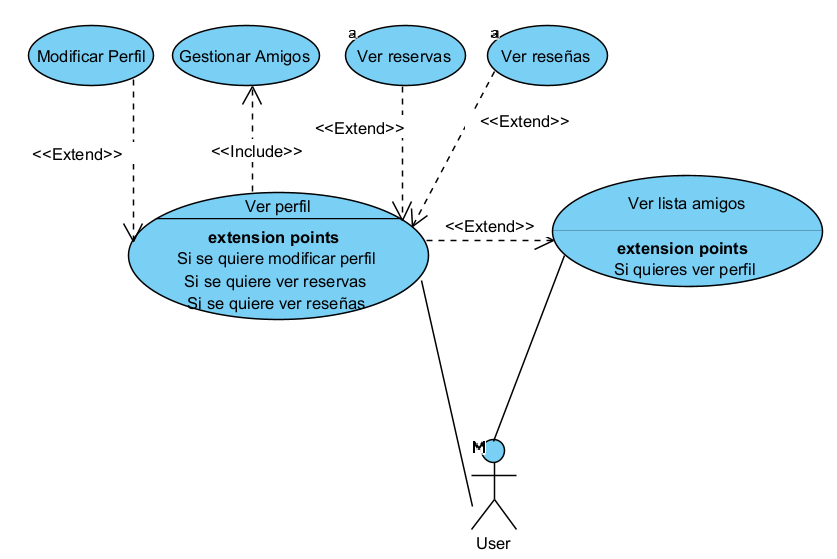
\includegraphics[width=0.8\textwidth]{./img/casos_uso/RedDeAmigos.png}
                \end{figure}\\
                \hline
                \textbf{Nombre:} Red de amigos.\\
                \hline
                \textbf{Descripción:} Permite al cliente gestionar su perfil, de modo que puede tanto consultar el historial de reservas y de reseñas, como añadir o eliminar amigos. También puede editar sus datos personales.\\
                \hline
                \textbf{Actores:} Usuario.\\
                \hline
                \textbf{Precondiciones:} Estar identificado en el sistema.\\
                \hline
                \textbf{Requisitos no funcionales:} Ninguno\\
                \hline
                \textbf{Flujo de Eventos:}
                \begin{enumerate}
                    \item El usuario puede consultar todo su historial de reservas realizadas en el sistema, pulsando en el botón “Consultar reservas”.
                    \item El usuario puede consultar todo su historial de reseñas realizadas en el sistema, pulsando en el botón “Consultar reseñas”.
                    \item El usuario puede añadir amigos pulsando en el botón “Agregar amigo”. Al pulsar el botón de “Agregar amigo” se abrirá un diálogo de texto donde podremos mandar una solicitud de amigo al usuario proporcionado.

                    \item El usuario puede borrar un amigo de la lista de amigos, seleccionando el nombre del amigo en la lista y pulsando el botón “Borrar amigo”. Al pulsar el botón de “Borrar amigo” se abrirá un Frame con un aviso para confirmar la acción.
                    \item El usuario puede editar los datos personales que desee pulsando en el botón “Editar perfil”. Al pulsar el botón de “Editar perfil” se abrirá un diálogo de texto en los datos personales donde podremos editarlos a nuestro gusto.  
                \end{enumerate}\\
                \hline
                \textbf{Poscondiciones:} Ninguna\\
                \hline
                \textbf{Interfaz Gráfica:}\\
                \begin{figure}[H]
                    \centering
                    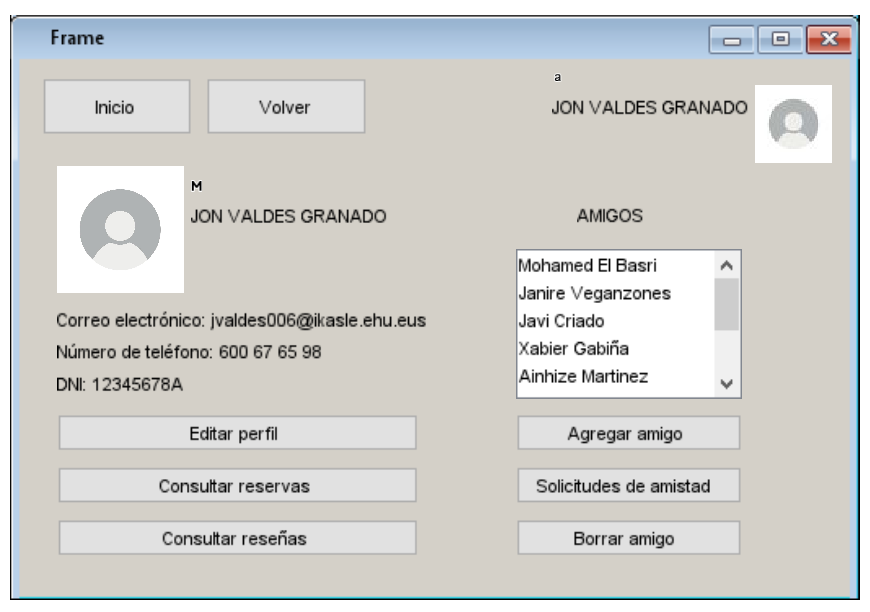
\includegraphics[width=0.8\textwidth]{./img/grafico/InterfazMenu.png}
                \end{figure}\\
                \hline
                \begin{figure}[H]
                    \centering
                    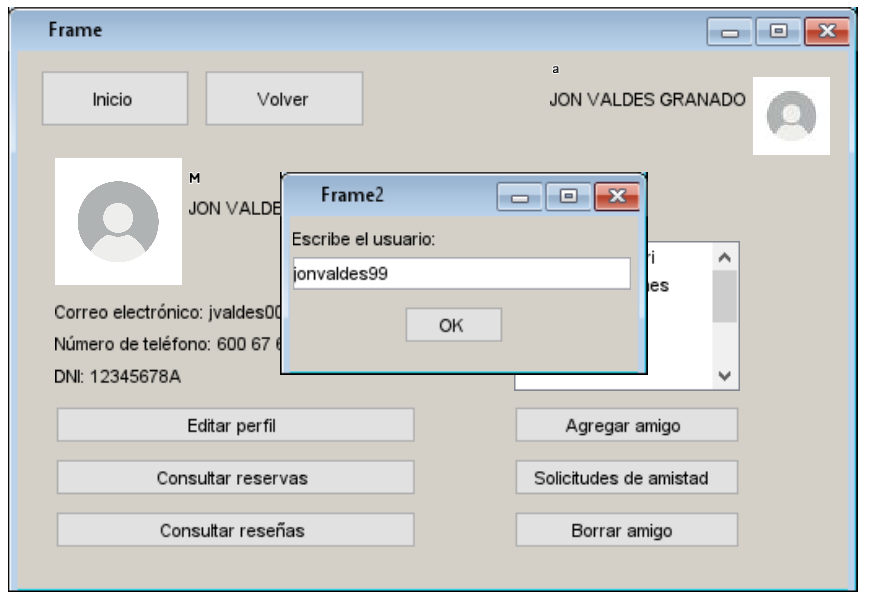
\includegraphics[width=0.8\textwidth]{./img/grafico/InterfazAnadrAmigo.png}
                \end{figure}\\
                \hline
                 \begin{figure}[H]
                    \centering
                    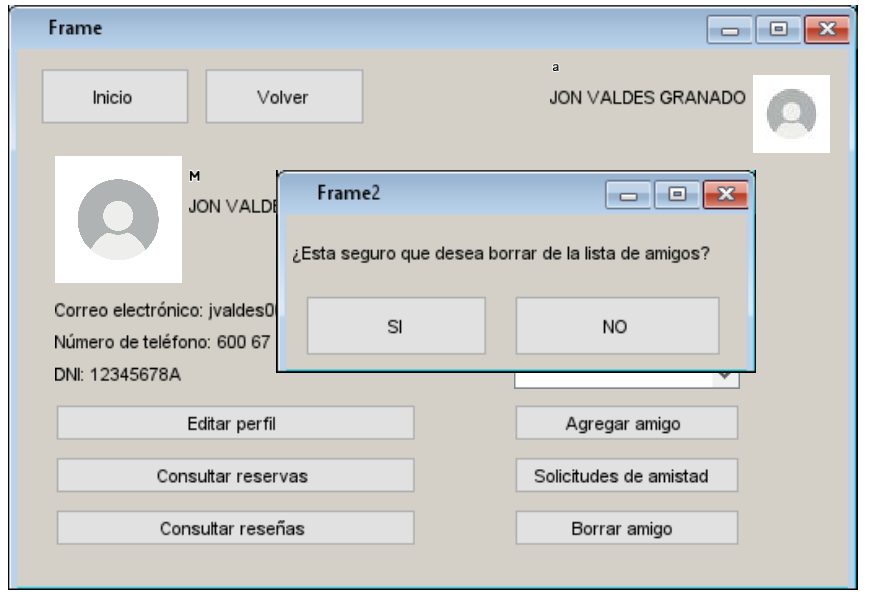
\includegraphics[width=0.8\textwidth]{./img/grafico/interfazAlertaBorrarAmigo.png}
                \end{figure}\\
                 \begin{figure}[H]
                    \centering
                    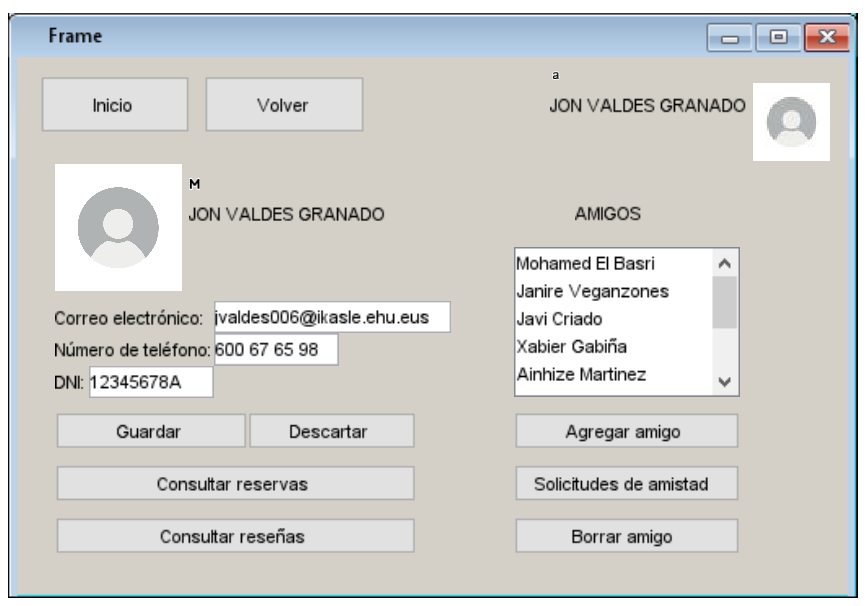
\includegraphics[width=0.8\textwidth]{./img/grafico/InterfazEditarPerfil.png}
                \end{figure}\\
            \end{longtable}
        \end{center}
        \clearpage
        \subsection{Administrador}
        \begin{center}
            \begin{longtable}{|p{\linewidth}|}
                \hline
                \textbf{Responsable:} Janire Veganzones\\
                \hline
                \begin{figure}[H]
                    \centering
                    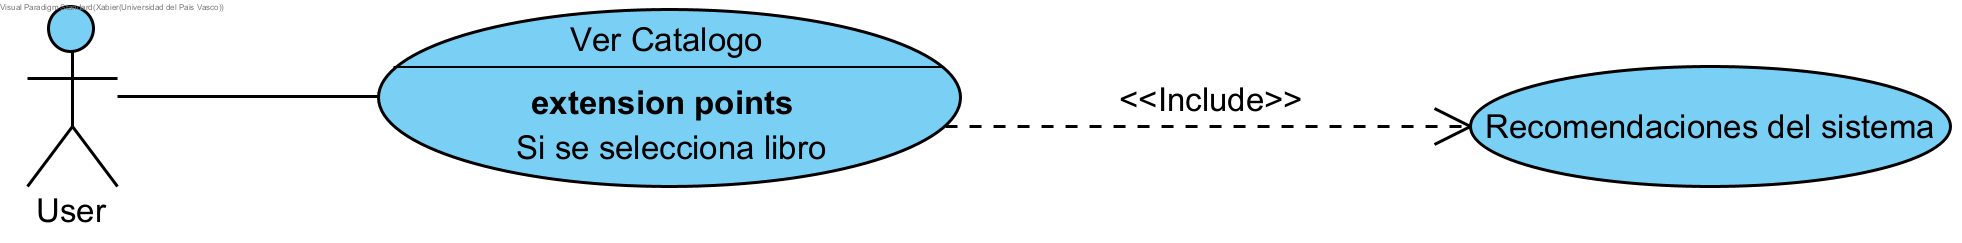
\includegraphics[width=0.8\textwidth]{./img/casos_uso/RecomendacionesLibros.png}
                \end{figure}\\
                \hline
                \textbf{Nombre:} Gestionar usuarios\\
                \hline
                \textbf{Descripción:}  Permite crear, eliminar o modificar un usuario en el sistema.\\
                \hline
                \textbf{Actores:} Admin\\
                \hline
                \textbf{Precondiciones:} Estar identificado en el sistema y ser usuario.\\
                \hline
                \textbf{Requisitos no funcionales:} Ninguno\\
                \hline
                \textbf{Flujo de Eventos:}
                \begin{enumerate}
                    \item El Usuario se identifica mediante su cuenta, en caso de ser un usuario administrador aparecerá el menú “Home” con el apartado de Administrador.
                    \item El usuario selecciona en su menú Home “Usuarios” para ver las funcionalidades que puede gestionar del usuario.
                    \item Se muestran las funcionalidades del usuario que puede gestionar el administrador.  
                    []
                \end{enumerate}\\
                \hline
                \textbf{Poscondiciones:} Ninguna\\
                \hline
                \textbf{Interfaz Gráfica:}\\
                \begin{figure}[H]
                    \centering
                    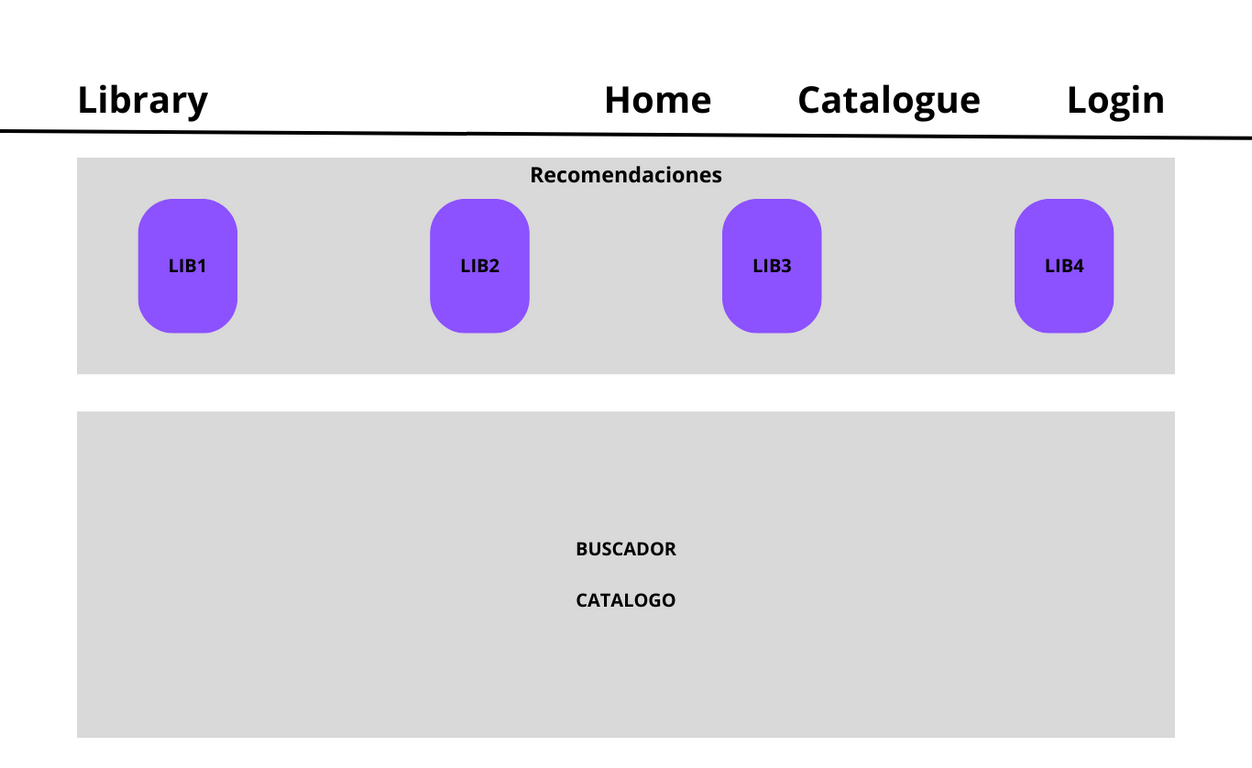
\includegraphics[width=0.8\textwidth]{./img/grafico/recom_lib.png}
                \end{figure}\\
                \hline
            \end{longtable}
        \end{center}
        \clearpage
        \subsection{Foros}
        \begin{center}
                \begin{longtable}{|p{\linewidth}|}
                    \hline
                    \textbf{Responsable:} Ainhize Martinez\\
                    \hline
                    \begin{figure}[H]
                        \centering
                        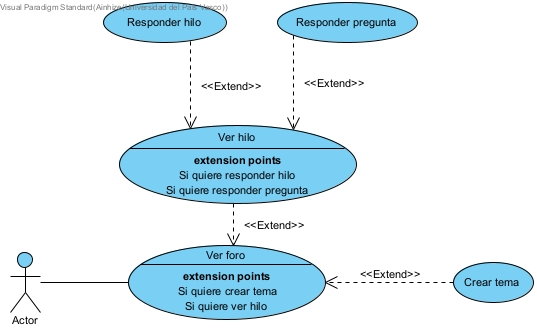
\includegraphics[width=0.8\textwidth]{./img/casos_uso/casos_foro.jpg}
                    \end{figure}\\
                    \hline
                    \textbf{Nombre:} Ver Foros\\
                    \hline
                    \textbf{Descripción:} Permite al usuario acceder al foro, crear temas nuevos, explorar todos los temas, además de hablar y contestar hilos.\\
                    \hline
                    \textbf{Actores:} Usuario\\
                    \hline
                    \textbf{Precondiciones:} Estar identificado en el sistema.\\
                    \hline
                    \textbf{Requisitos no funcionales:} Ninguno\\
                    \hline
                    \textbf{Flujo de Eventos:}
                    \begin{enumerate}
                        \item[1.] El usuario selecciona "Foro" para acceder a él.
                        \item[2.] Se le muestra toda la lista de temas.
                        \newline
                        \newline
                        [Si el usuario accede a un tema] 
                        \begin{enumerate}
                            \item[3a.] El usuario puede hablar o contestar un tema.
                        \end{enumerate}
                        [Si el usuario pulsa sobre "+tema"]
                        \begin{enumerate}
                            \item[3b.] Se añade un nuevo tema
                        \end{enumerate}
                    \end{enumerate}\\
                    \hline
                    \textbf{Poscondiciones:} Ninguna\\
                    \hline
                    \textbf{Interfaz Gráfica:}\\
                    \begin{figure}[H]
                        \centering
                        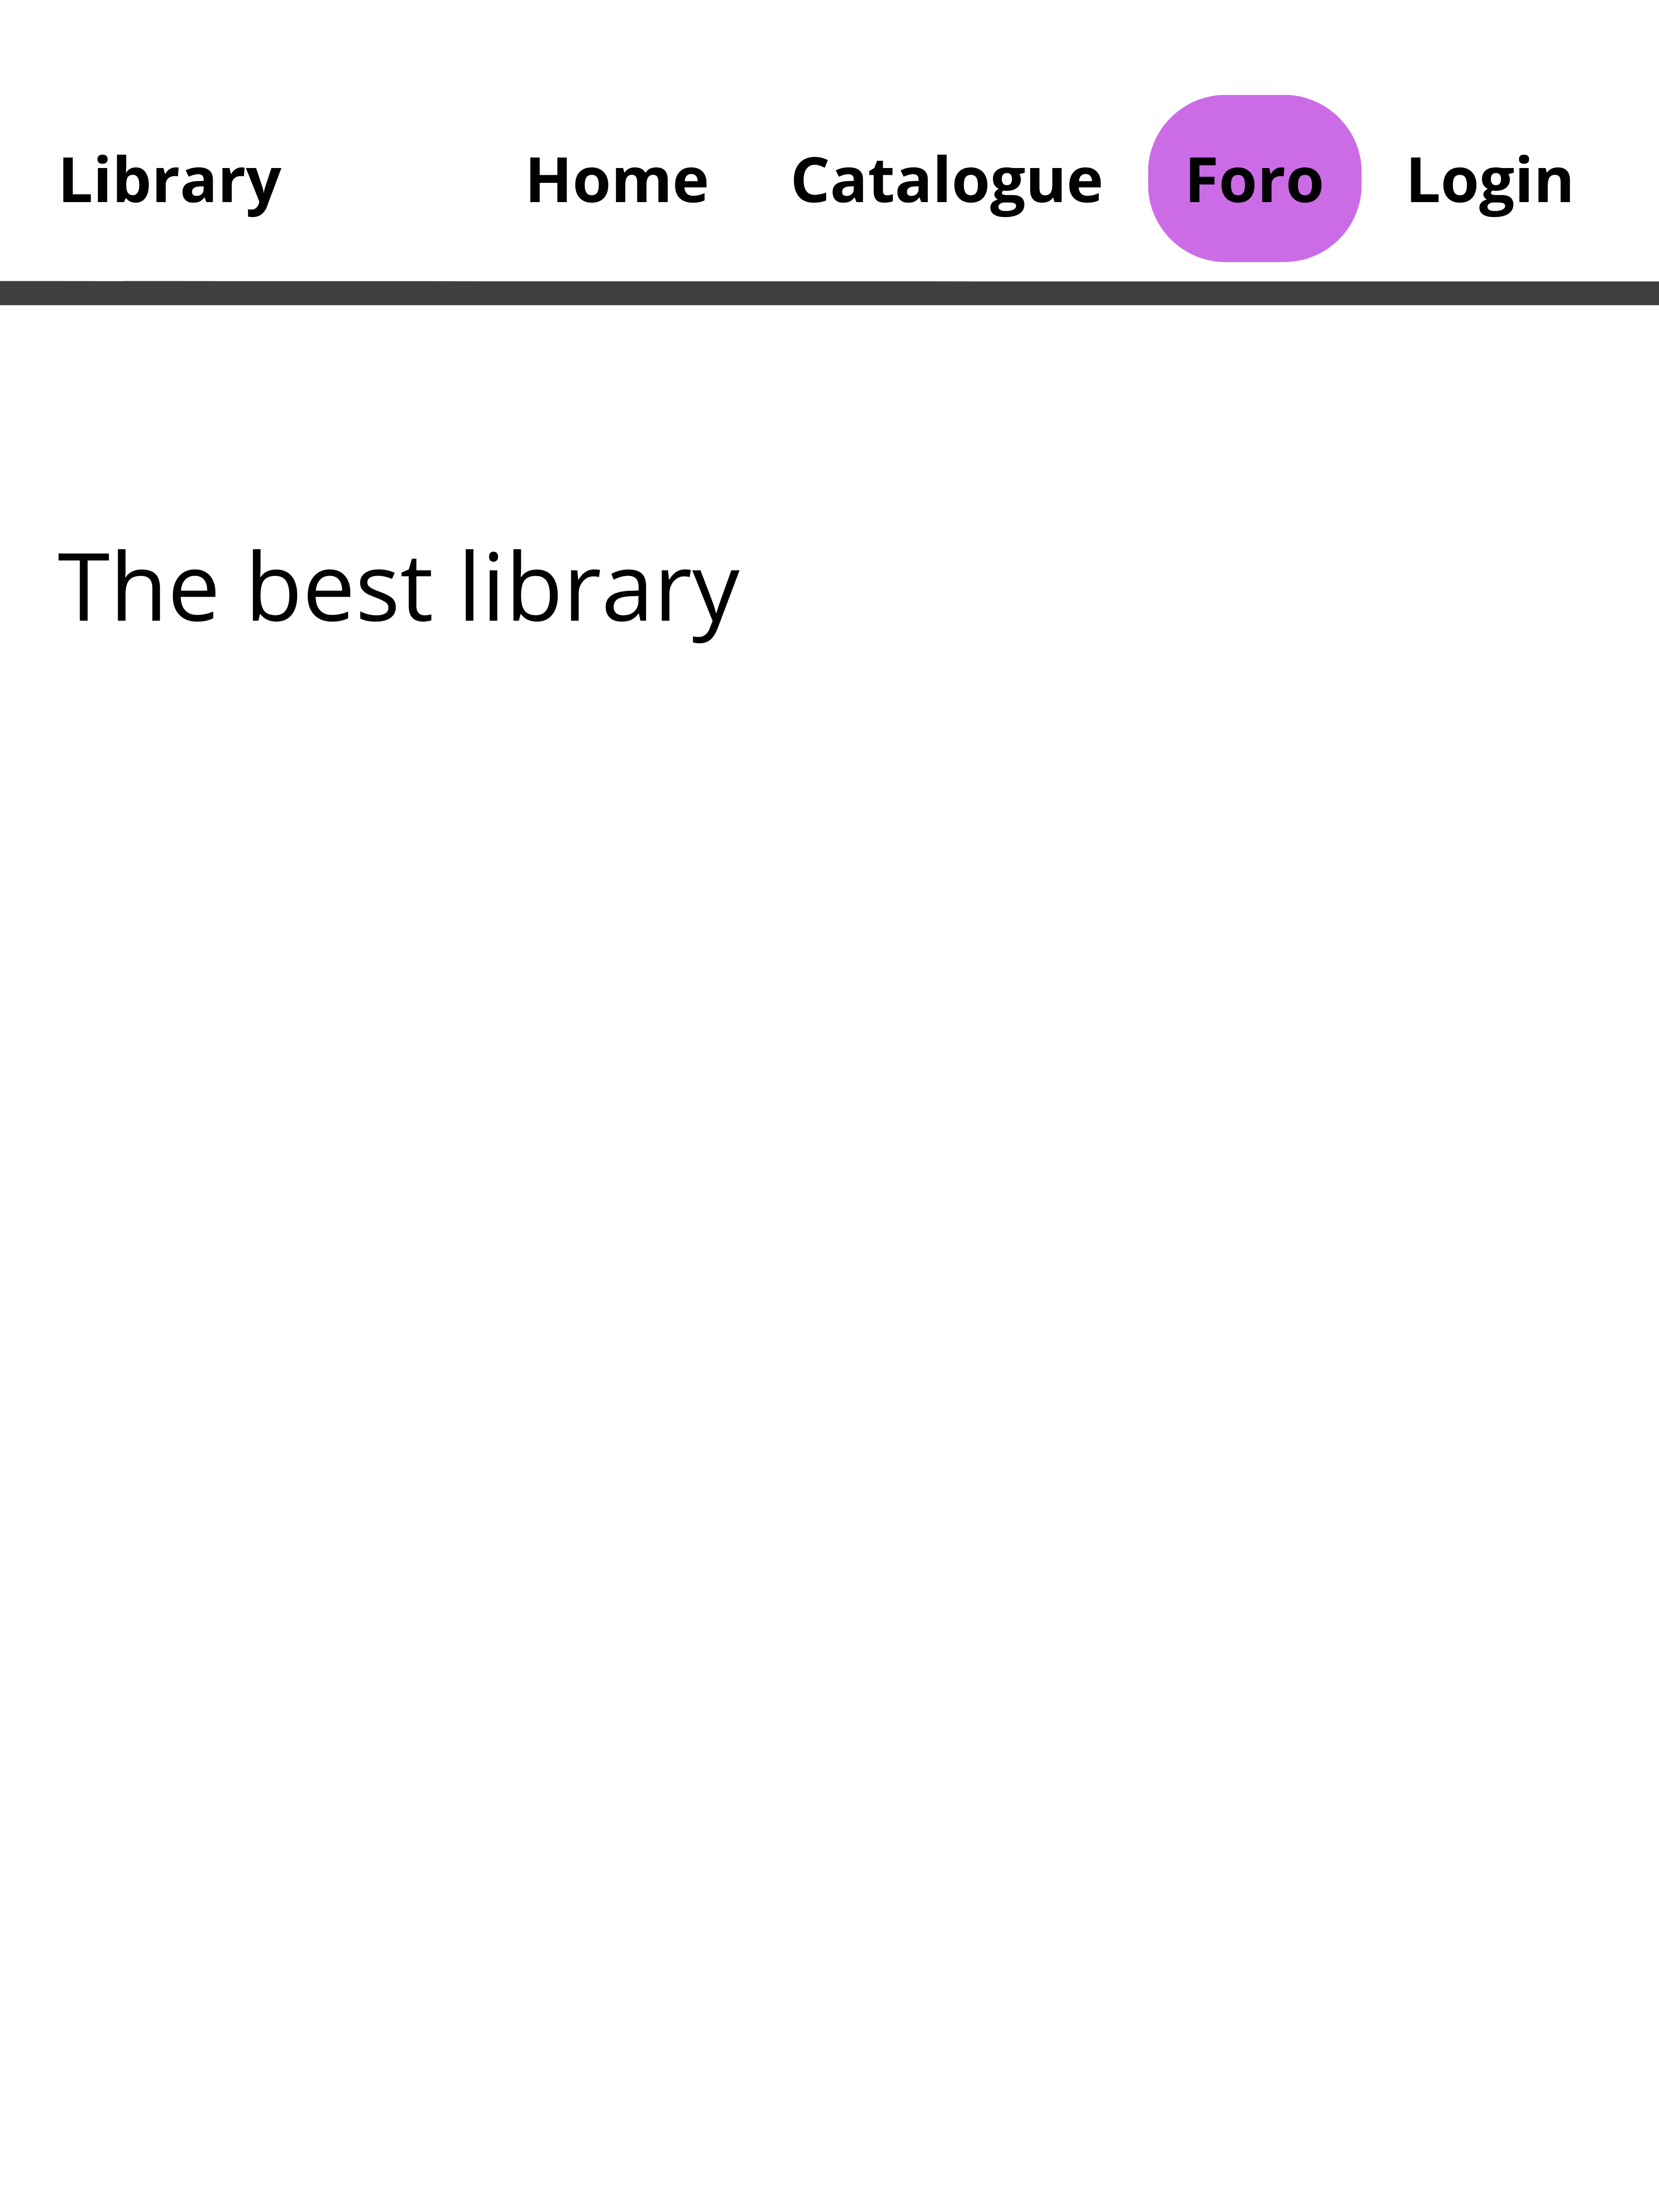
\includegraphics[width=0.8\textwidth]{./img/grafico/Foro1.png}
                    \end{figure}\\
                    \hline
                    \begin{figure}[H]
                        \centering
                        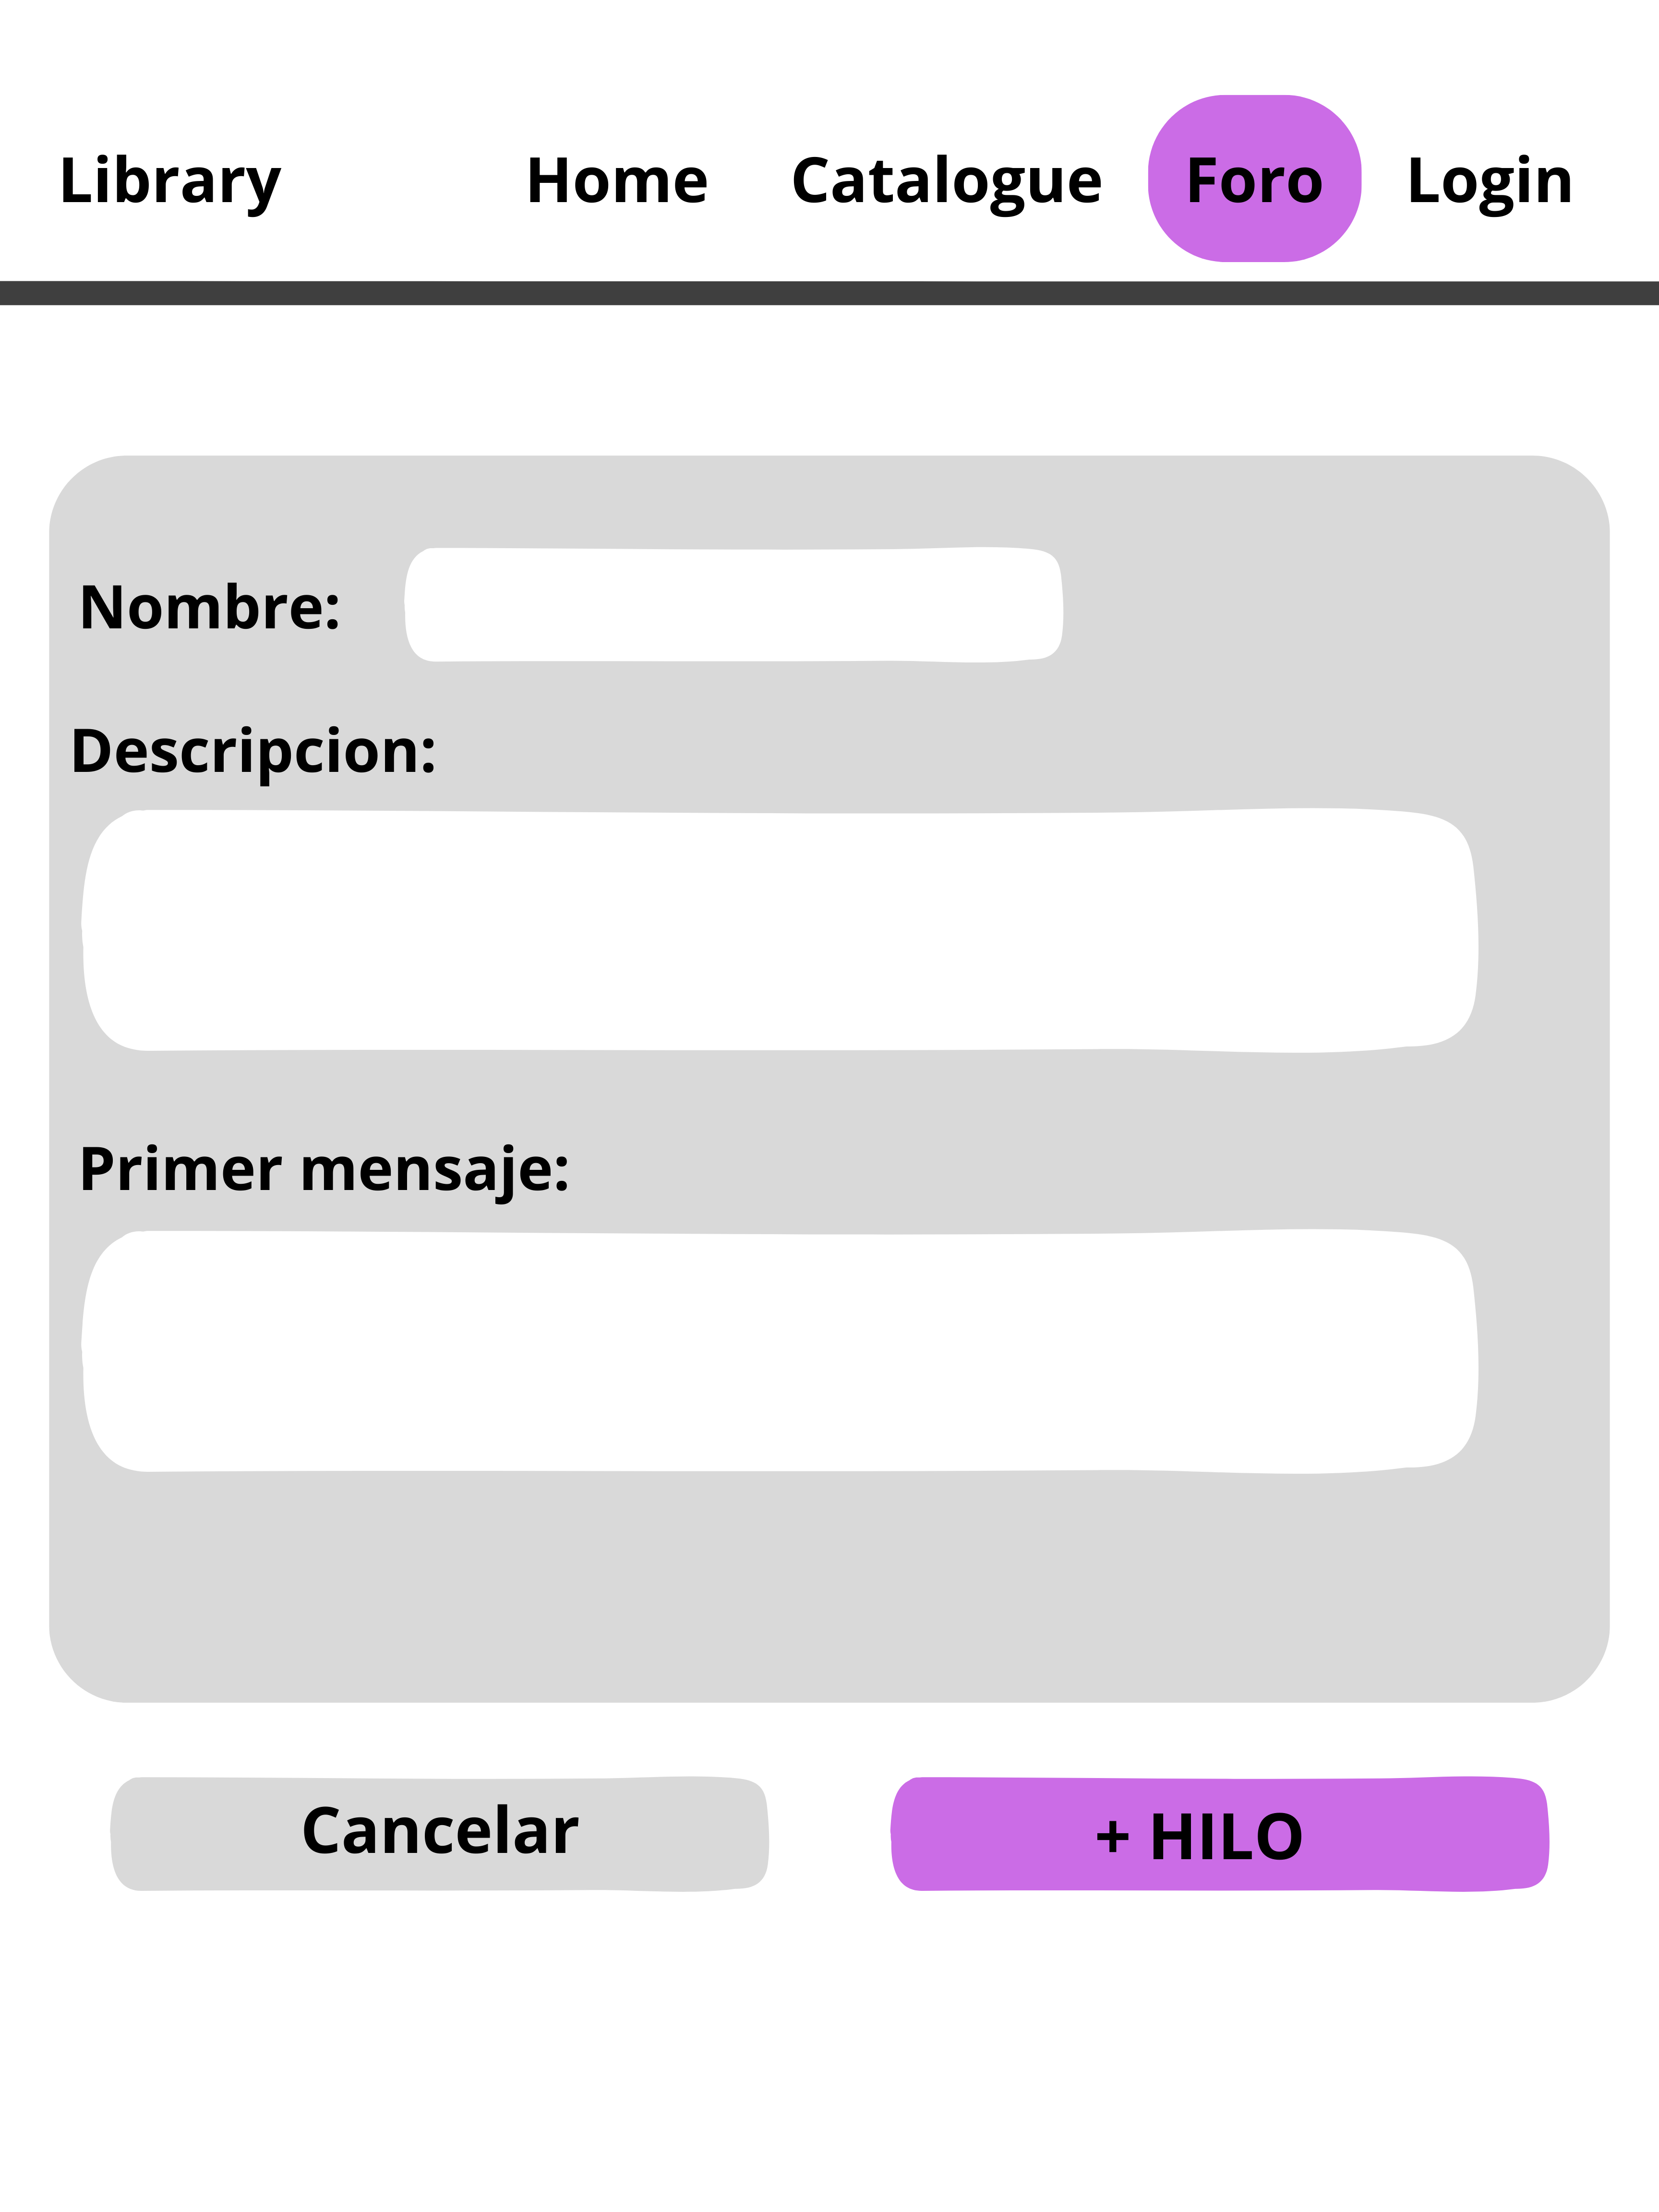
\includegraphics[width=0.8\textwidth]{./img/grafico/Foro2.png}
                    \end{figure}\\
                    \hline
                    \begin{figure}[H]
                        \centering
                        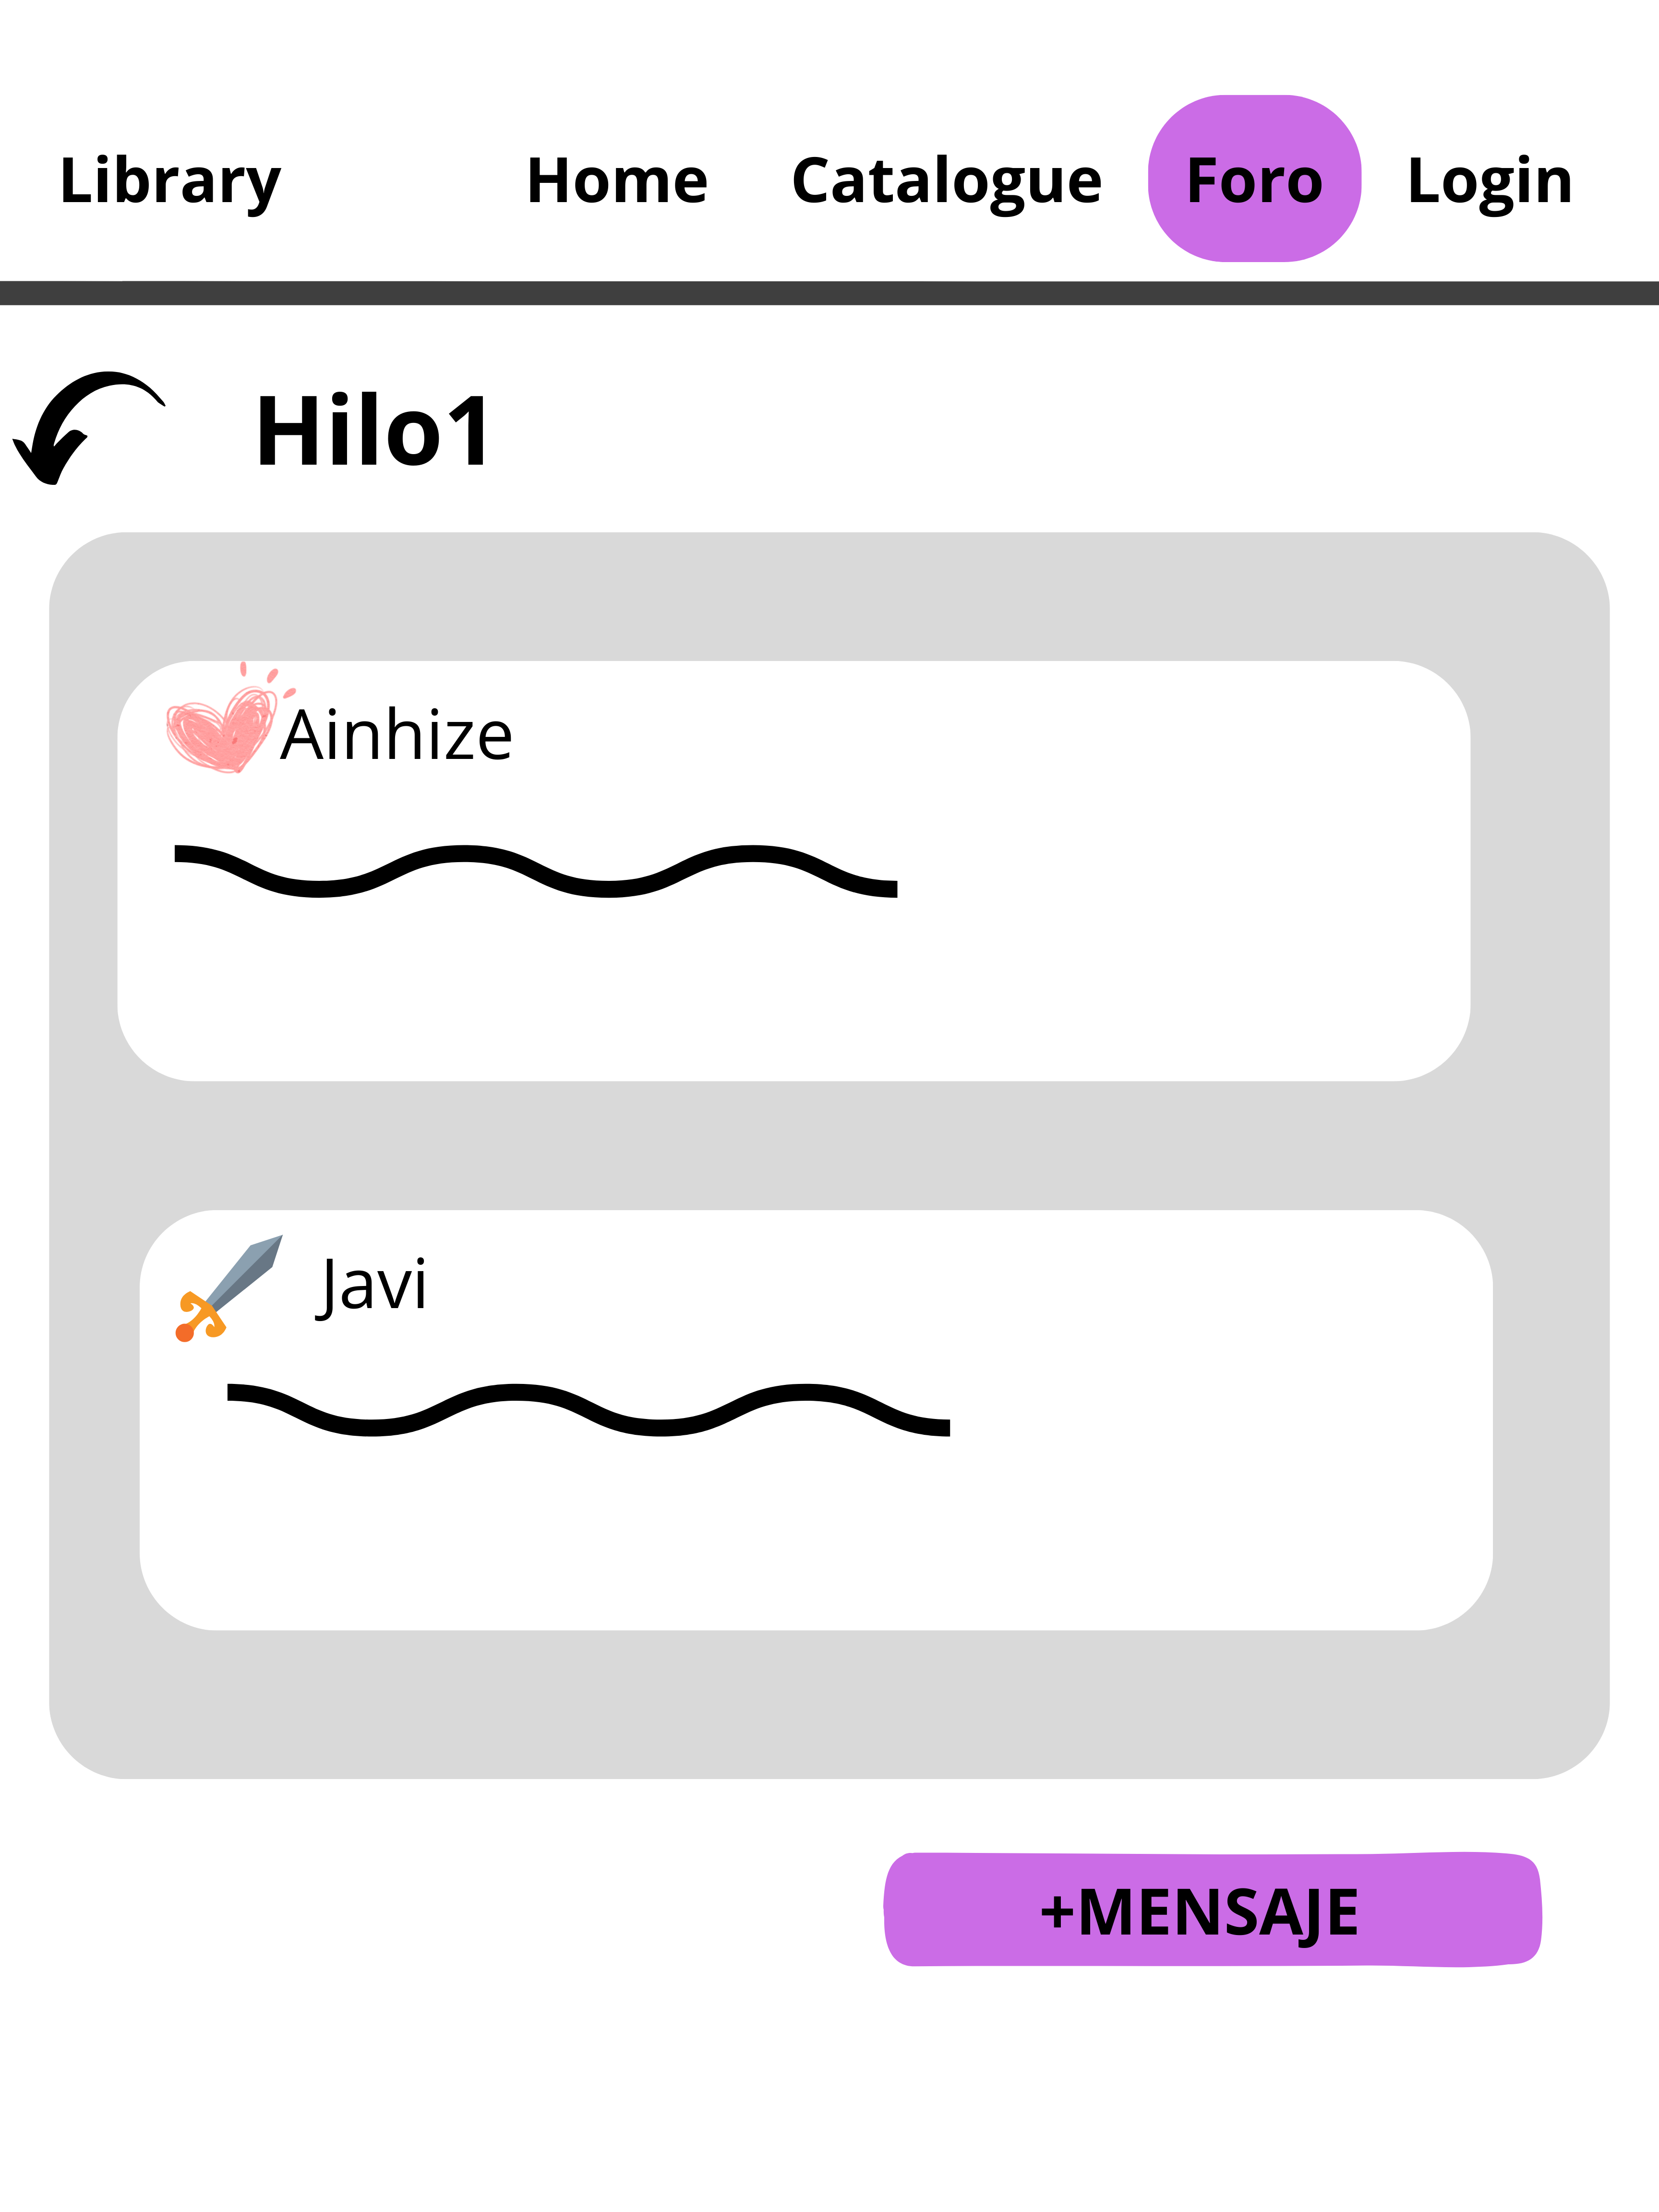
\includegraphics[width=0.8\textwidth]{./img/grafico/Foro3.png}
                    \end{figure}\\
                    \hline
                    \begin{figure}[H]
                        \centering
                        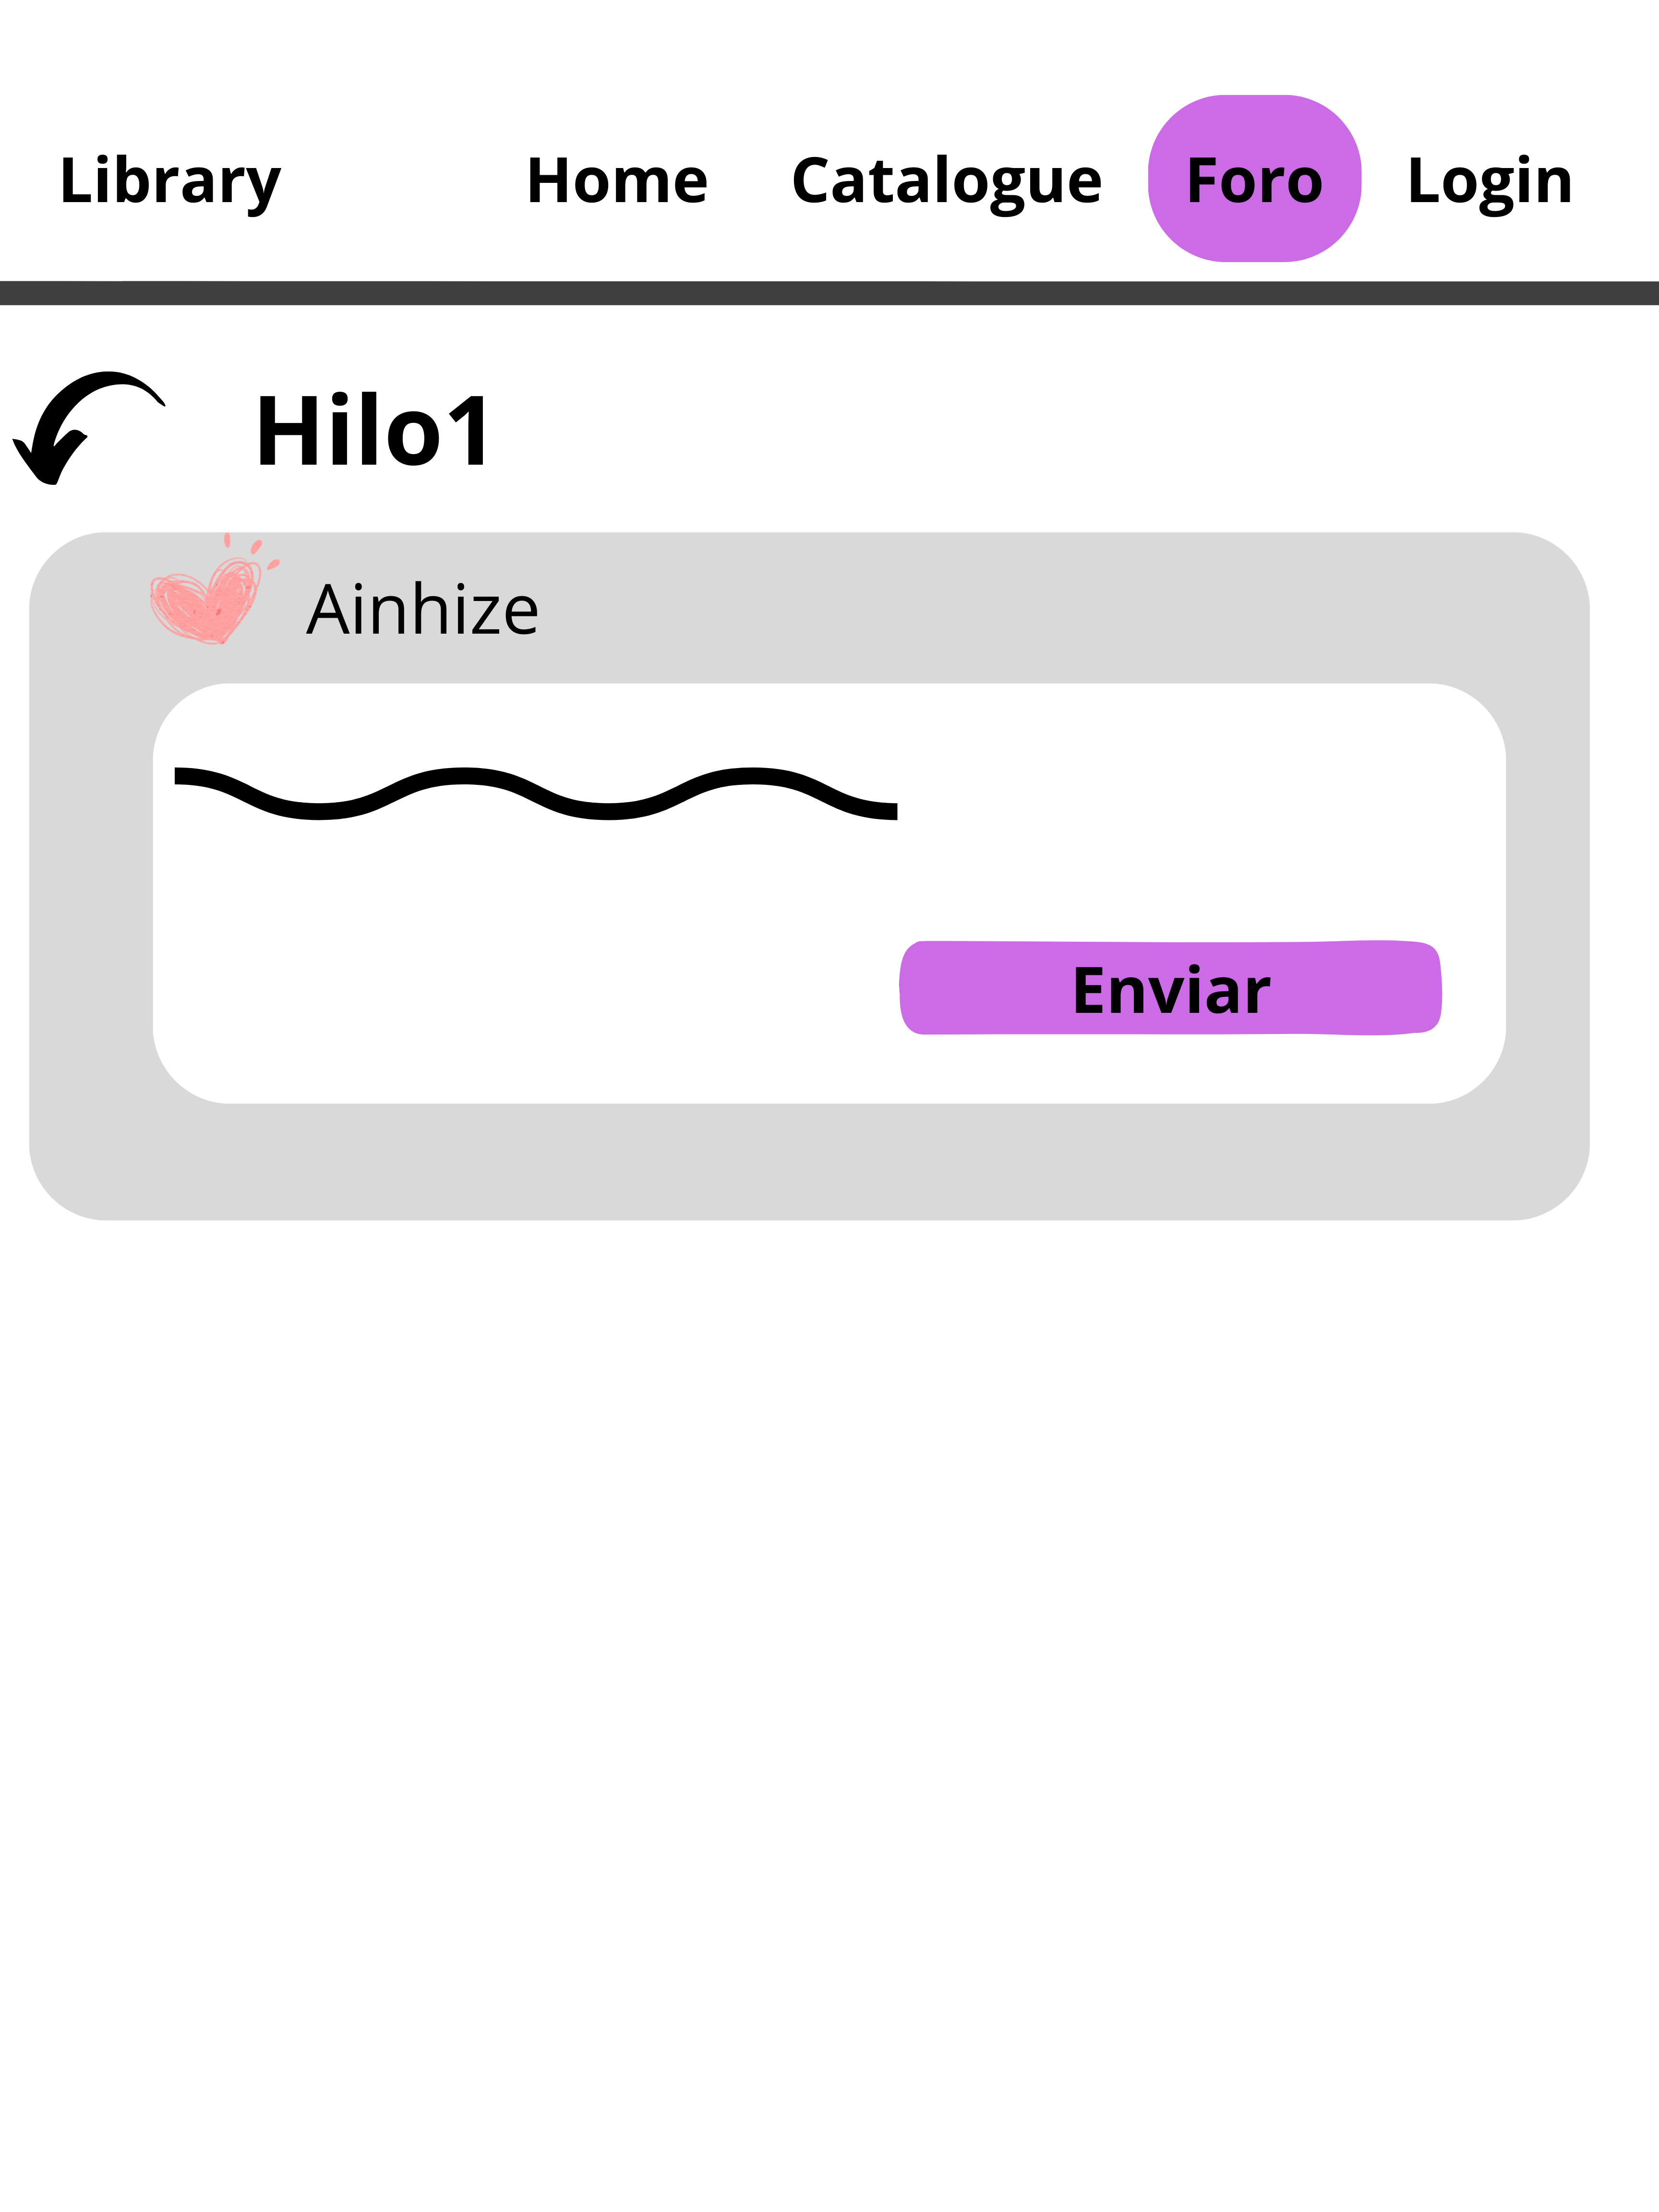
\includegraphics[width=0.8\textwidth]{./img/grafico/Foro4.png}
                    \end{figure}\\
                    \hline
            \end{longtable}
        \end{center}
        \clearpage
        \subsection{Recomendaciones del sistema}
            \begin{center}
                \begin{longtable}{|p{\linewidth}|}
                    \hline
                    \textbf{Responsable:} Xabier Gabiña\\
                    \hline
                    \begin{figure}[H]
                        \centering
                        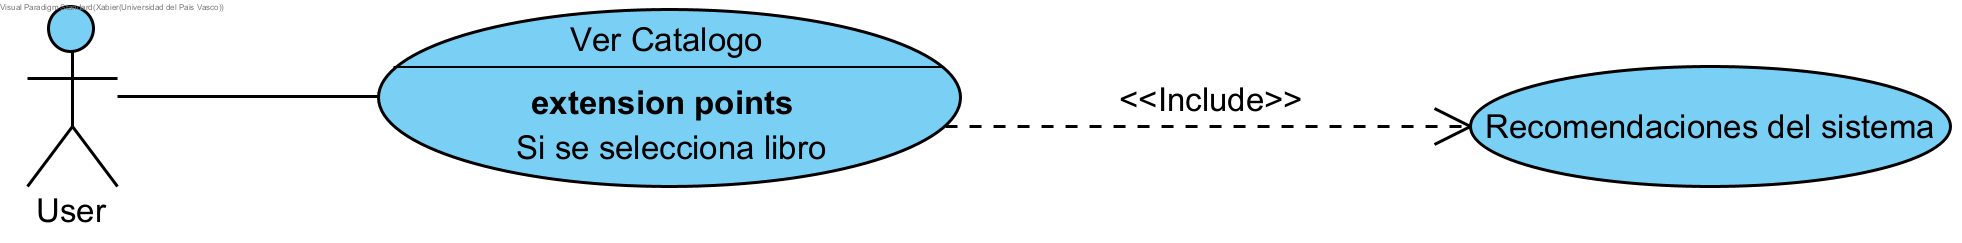
\includegraphics[width=0.8\textwidth]{./img/casos_uso/RecomendacionesLibros.png}
                    \end{figure}\\
                    \hline
                    \textbf{Nombre:} Ver libros recomendados\\
                    \hline
                    \textbf{Descripción:} Muestra una lista en la parte superior del catálogo mostrando los libros con más préstamos del sistema en funcion de los gustos del usuario.\\
                    \hline
                    \textbf{Actores:} Usuario\\
                    \hline
                    \textbf{Precondiciones:} Estar identificado en el sistema y haber tenido un libro registrado\\
                    \hline
                    \textbf{Requisitos no funcionales:} Ninguno\\
                    \hline
                    \textbf{Flujo de Eventos:}
                    \begin{enumerate}
                        \item El Usuario entra en el catalogo para ver las peliculas disponibles.
                        \item Se le muestra en la parte superior de la pantalla una serie de peliculas basadas en los generos y peliculas que consume el usuario.
                    \end{enumerate}\\
                    \hline
                    \textbf{Poscondiciones:} Ninguna\\
                    \hline
                    \textbf{Interfaz Gráfica:}\\
                    \begin{figure}[H]
                        \centering
                        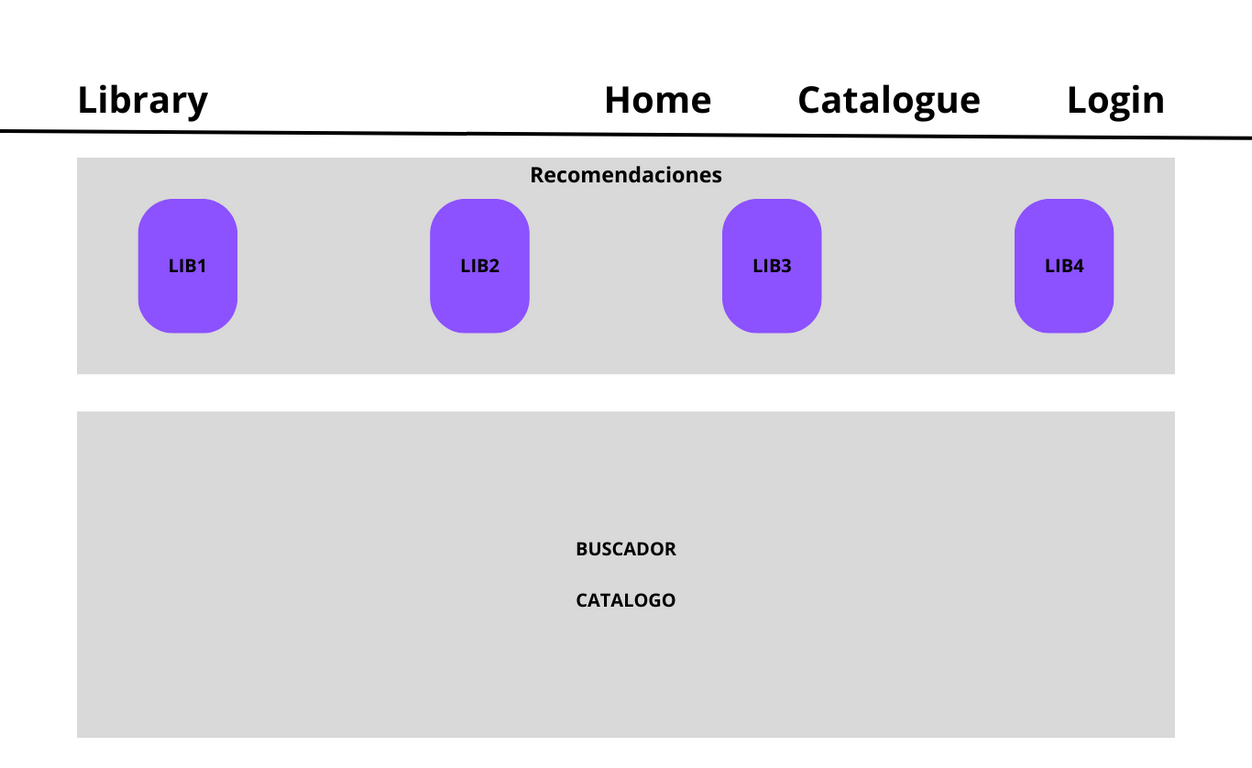
\includegraphics[width=0.8\textwidth]{./img/grafico/recom_lib.png}
                    \end{figure}\\
                    \hline
                \end{longtable}
            \end{center}
        \clearpage
        \subsection{Recomendaciones de amigos}
    \chapter{Conclusiones} 
\end{document}
